\documentclass{bioinfo}
\copyrightyear{2005}
\pubyear{2005}

\begin{document}
\firstpage{1}

\title[Supplementary information - The Functional Therapeutic Chemical Classification System]{Supplementary information - 
The Functional Therapeutic Chemical Classification System}

\section*{Availability and Implementation}

This section describes the building mechanism behind the FTC. 
First, a list of categories describing the mode and mechanism of action of drugs is defined. 
Then in a second step the newly created categories are automatically populated with approved compounds. 
Finally, the FTC is evaluated and repurposing hypotheses can be generated.

\section{Source code}
The code behind the creation of the resource is entirely open and available 
at {{https://github.com/loopasam/ftc}}. The web application built on the top of the 
FTC can be find at {{https://www.ebi.ac.uk/chembl/ftc}} and the documentation can be 
accessed at {{https://github.com/loopasam/ftc/wiki}}. The reader should be familiar with 
description logics and the Web Ontology Language (OWL) to fully understand the construction of the 
knowledge base. An introduction to description logics from the perspective of the biomedical scientist is 
available on the wiki at {{https://github.com/loopasam/ftc/wiki/Description-Logics}}. The FTC implementation 
relies mostly on Brain \citep{Croset2013} and the web application builds on the top of the Play! framework. 
Classification tasks use the ELK reasoner \citep{Kazakov2011}. The computer hosting the web application has 8 Gb of memory 
with 4 processors, this architecture allows fast parallel reasoning, thanks to ELK's design. More functionalities 
will be added to the web application following user requirements (so called \emph{lean implementation}).

\section{FTC categories creation}
The mode of action categories present in the FTC are defined based on the terms coming from the 
Gene Ontology (GO) \citep{Ashburner2000}. Both the molecular function and biological process branches are used for 
this purpose, yet handled differently.

\subsection{Categories related to biological processes}
All the biological processes featured by the GO are looked-up one by one. All the 
time a process is linked to another process (\emph{X}) via a \emph{positive} or \emph{negative regulation} link, two FTC 
classes are created: \emph{Anti-X agent} and \emph{Pro-X agent}. For instance the GO term \emph{positive regulation of blood 
coagulation} is linked to the term \emph{blood coagulation} via a \emph{positively regulates} relation, therefore two FTC 
categories \emph{Anti-blood coagulation agent} and \emph{Pro-blood coagulation agent} are created. The identifiers of the 
new FTC classes are also derived from the GO term used to create the class pattern. The GO numeric identifier 
is re-used and the letter \emph{A} or \emph{P} is appended before to emphasize the \emph{anti} or \emph{pro} pattern. 
From the example presented 
previously, the FTC class \emph{Anti-blood coagulation} has FTC\_A0007596 as identifier, because the GO term \emph{blood coagulation} is 
referenced by GO:0007596. Following the same logic, FTC\_P0007596 is the identifier of the class \emph{Pro-blood coagulation agent}. The 
design choice for identifiers and labels allows the FTC to fully rely on the high quality work provided by the GO curation 
team and scale over it.

\subsection{Categories related to molecular functions}
The mode and mechanism of actions related to molecular functions are created in the following manner: All the time 
a molecular function (\emph{Y}) is encountered then two FTC categories are created, as for the processes: \emph{Anti-Y agent} and 
\emph{Pro-Y agent}. The identifiers are assigned the same way as described before. For instance, out of the GO term \emph{androgen 
receptor activity} (GO:0004882) two FTC classes are derived: \emph{Pro-androgen receptor activity agent} (FTC\_P0004882) and 
\emph{nti-androgen receptor activity agent} (FTC\_A0004882).


\section{Equivalent definitions}
FTC classes are generated as presented in the previous section. Up to this point, these categories 
are only tokens with a human readable label as well as an identifier. The next step is going to 
assign equivalent definitions to each FTC class. A reasoner can understand such definitions and will automatically 
classify the knowledge base accordingly; drugs will then be assigned to FTC categories and the taxonomic structure 
arises after this reasoning step. Equivalent definitions are written as OWL class expressions using the entities of 
the knowledge base (summarised at {{https://github.com/loopasam/ftc/wiki/Knowledge-Base}} and in section ).

//TODO refer to section

There are two types of equivalences: The first one captures perturbation of regulatory 
biological processes (so called regulatory patterns) and the second one handles the perturbed functions (functional patterns).

\subsection{Regulatory pattern}
Some of the FTC categories are created from the biological processes present in the 
GO (cf previous sections); these categories have two arbitrary equivalent definitions, representing the 
two possible ways a compound might impact the biological process. Anti-biological process agent FTC categories 
contain the drugs that negatively perturb a target involved in the positive regulation of the biological process. 
The anti categories also feature the compounds that positively perturb a negative regulator of the same process. 
The pro categories are equivalent to the opposite pattern. Figure 5 illustrates the equivalent definitions for the 
FTC class Anti-blood coagulation agent (FTC\_A0007596).
 
\begin{figure}[!tpb]%figureS1
\centerline{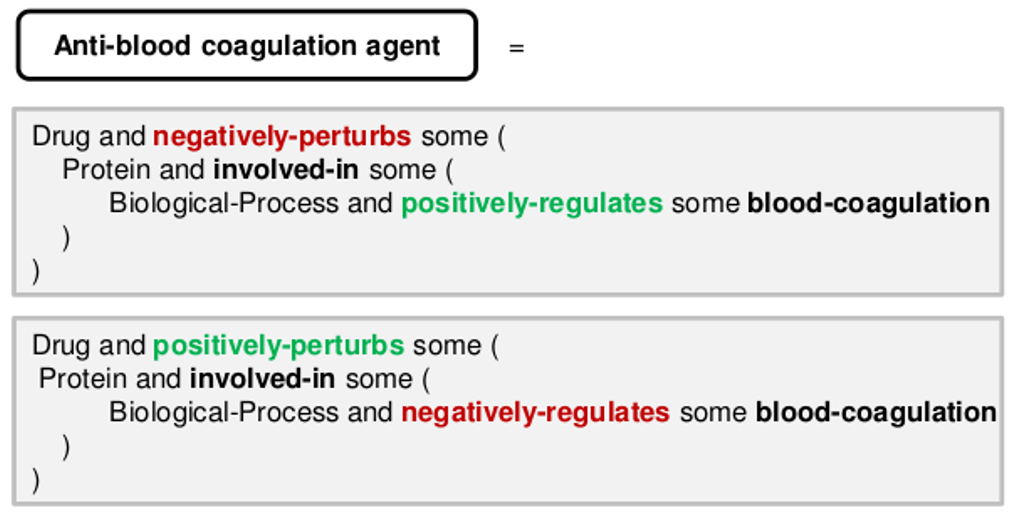
\includegraphics{figS1.png}}
\caption{Example of equivalent definitions (gray boxes) for the FTC category Anti-blood coagulation 
agent (FTC\_A0007596). After the data integration step, a reasoner will look the definitions and identify 
which drugs comply with the FTC definitions. Definitions are expressed using the Web Ontology Language (OWL), 
serialised here using the Manchester syntax.}\label{fig:S01}
\end{figure}

\subsection{Functional pattern}
The FTC categories generated from the GO molecular functions are also equivalent to a logical 
definition. Anti FTC categories dealing with molecular activities are asserted as equals to the drugs 
that negatively perturb the function. Pro categories are equivalent to the drugs that positively perturb the 
function of interest. A summary of the patterns definitions is available on the 
online wiki at {{https://github.com/loopasam/ftc/wiki/Mode-of-Action}}.

\section{Data integration}
At this stage, the knowledge base contains the created FTC classes associated with their 
logical definitions, as well as the GO and the core FTC entities. The knowledge base is then 
further populated with some information coming from various public databases. Only manually curated 
information is considered. This section illustrates how the core entities interact with the different data types 
in order to create the axioms.

\subsection{DrugBank}
The DrugBank database is a unique bioinformatics and cheminformatics resource 
that combines detailed drug data with comprehensive drug target information \citep{Knox2011}. The approved 
drugs (small molecules and biotherapeutics) acting on proteins are extracted from the database and 
imported in the FTC knowledge base. In order to be selected, a compound must firstly be approved and 
secondly have a pharmacological action on at least one human protein target present in Uniprot \citep{TheUniprotConsortium2013}. 
The protein targets all have at least one manually asserted GO annotation \citep{Dimmer2012} for a biological process or a 
molecular function. DrugBank links compounds to targets via actions. The DrugBank actions are somehow 
structured and consistent: Concepts such as inhibitor or agonist are reused throughout the database for 
example, yet they are not strictly formalised as a controlled vocabulary. These actions are manually 
standardised to the core properties of the FTC according to their meaning: For instance the action 
antagonist is mapped to the FTC negatively-perturbs.
Compounds coming from DrugBank are represented as OWL classes and asserted 
as subclasses of DrugBank compound (FTC\_C2). Protein targets are described as classes 
too and subclasses of the core class protein. Each DrugBank compound is then connected to 
its target via the following axiom pattern: \emph{drug SubClassOf perturbs some protein}. 
E.g. \emph{Ximelagatran SubClassOf negatively-perturbs some Prothrombin}.

\subsection{Gene Ontology annotations}
The GO annotation program aims to provide high-quality GO annotations to 
proteins in UniProt. In the context of the FTC, such annotations are used 
to create axioms linking protein targets to molecular functions and biological processes. 
Each protein annotated with a function creates an axiom such 
as protein SubClassOf has-function some molecular function. 
Each protein annotated to a biological process creates an axiom such 
as protein SubClassOf involved-in some biological process. 
E.g. Prothrombin SubClassOf involved-in some positive regulation of blood coagulation. 
Each protein can be involved in multiple processes and capable of realizing multiple functions.

\section{Knowledge base classification}
The knowledge base is fully built at this step and contains core classes, mode 
of actions descriptions alongside the actions of approved DrugBank compounds on 
protein targets in Uniprot. The proteins are linked to their molecular functions and involvement in 
biological processes via the GO annotations. The logical specifications of the FTC are there to glue 
the different data together and to explicitly express the logical links between resources. The FTC 
knowledge base follows an OWL2 EL profile, which enable the use of fast and parallelised reasoners such 
as ELK (cite). During the classification process, the reasoner checks whether the mode of action equivalent 
definitions are satisfied or not and assigns drugs inside the corresponding FTC categories. The tree structure 
of FTC appears also at this step from the logical definitions.

\section{Evaluation methodology}
As the classification of therapeutic agents is done in an automated way, it 
is important to evaluate the results generated against a known resource which will be 
considered as gold standard. The assessment of the FTC is done against another similar 
classification, the Anatomical Therapeutic Chemical Classification System (ATC) \citep{world2000anatomical}). 
The ATC has been developed to serve as a tool for drug utilization research in order to 
improve quality of drug use. In this resource, the information is manually curated, and drugs 
are assigned to categories based of their legally approved indications. The goal of the ATC differs 
from the one of the FTC, yet the two resources are sharing some very similar concepts, which can be 
used for the evaluation. Categories of both classifications contain approved drugs with a DrugBank 
identifier, meaning that some of the drugs indexed in the FTC are also present in the ATC. From that, 
it is possible to define some evaluation points, which will help to assess the automated classification process.

\subsection{Evaluation Points}
An evaluation point is defined as an equivalence between a class from the FTC with one or 
more classes from the ATC. The idea is to look at the set of drugs contained in both side of the 
equivalence and estimate the overlap. This is illustrated in the Figure 6. Evaluation points are defined 
by hand and not themselves evaluated. The full list of evaluation points as well as a summary of the results 
are available online at https://www.ebi.ac.uk/chembl/ftc/evaluation/. Each evaluation point has a series of 
true/false positive and false negative drugs associated with it.
 
\begin{figure}[!tpb]%figureS2
\centerline{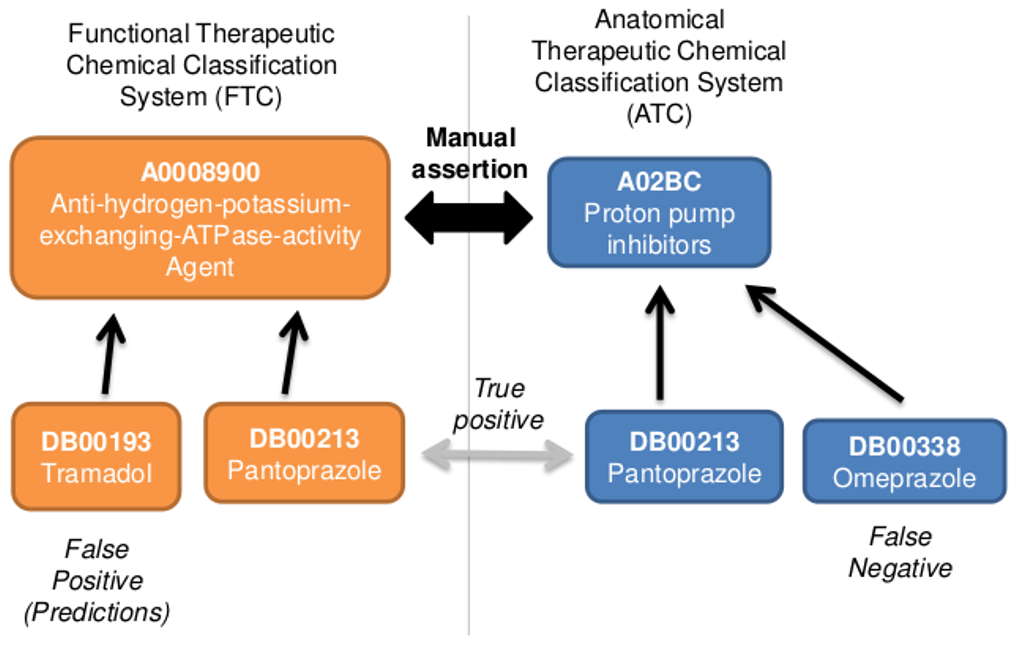
\includegraphics{figS2.png}}
\caption{Example of evaluation point. Classes from the ATC are manually 
mapped to classes from the FTC. The drugs present in each side of the equivalences 
are compared, and some metrics are derived from it (false positive/negative and true positive). 
A summary of the evaluation is available online at {{https://www.ebi.ac.uk/chembl/ftc/evaluation/}}.}\label{fig:S02}
\end{figure}

\subsection{True Positives}
Drugs that are present in both the FTC and the equivalent ATC class(es) are called true positives. 
These compounds reflect that the automated classification was capable of retrieving correctly the 
information present in the gold standard (ATC).

\subsection{False Negatives}
These drugs are present in the ATC class(es) but not in the corresponding FTC class. 
The automated classification failed to retrieve these compounds. The smaller the number of 
false negatives is, the better the FTC is at recalling drugs. A small number of false negatives 
means that if a drug is present in the ATC (gold standard), then it is likely that this drug will 
also be correctly categorised in the FTC.

\subsection{False Positives}
The false positives are the drugs present in the FTC category of the evaluation point but not in the corresponding ATC classes. 
A high number of false positives means that the FTC is over-assigning compounds to classes.
The false positives relates to the accuracy of the classification. In the context of this work, 
some false positives could also be considered as drug repurposing opportunities.

\subsection{Precision}
Precision is the probability that a randomly selected drug from the FTC is present in the equivalent ATC classes. 
The value is standardised as a percentage and corresponds to the formula: True Positive / (True Positive + False Positive).

\subsection{Recall}
Recall is the probability that a randomly selected drug from the ATC has been assigned to the correct 
corresponding class in the FTC. The value is standardised as a percentage and corresponds 
to the formula: True Positive / (True Positive + False Negative).

\section{Semantic similarity}
The semantic similarity measure performed over the FTC is a derivative of the Jaccard index \citep{jaccard1912distribution} \citep{rogers1960computer}. 
It is probably best understood as an example: If we consider two classes A and B, the semantic similarity 
between these classes corresponds to the number of OWL superclasses (direct and indirect, obtained with a reasoner) that 
are shared by A and B (intersection) divided by the number of superclasses of A or B (union). The index ranges 
from 0 (totally different) to 1 (identical).

\section{Mode of action similarity against indication}
A statistical analysis was performed over the data presented on Figure 3. 
When two compounds are randomly taken, they have on average a higher mode of action similarity when 
they are assigned to the same ATC category (one ATC level). In order to estimate whether this observation was 
due to chance only, we formulated the following null hypothesis (H0): For a pair of drug A and B, it does not 
matter to which ATC category they belong to, the average similarity is always the same. 
The alternative hypothesis (H1) was: For a pair of drug A and B, if A and B have the same ATC code, 
we expect on average to obtain a higher similarity value than if A and B have different ATC codes. 
A permutation test was then performed for each ATC category. For example, we started with the ATC 
category A (first row on Figure 3), looked at the similarity values when pairs of compounds both belong 
to the category A (top right corner square) and compared it to the similarity values when the pair of compounds 
belong to different categories (A and B, A and C and so forth). For each comparison we obtain two distributions of 
values (not shown). On average the similarity values are always higher when the two compounds 
belong to the same category (A/A versus A/B for instance). A permutation test (n = 20'000) was 
performed in order to see whether this observation was due to chance only. We were able to reject the null 
hypothesis for a significance level of 0.05 all the times. As the test is performed multiple times, 
we applied a Bonferroni correction for multiple hypothesis testing, which changed the significance level accordingly. 
The choice for a permutation test was driven by the fact that MoA similarity values do not follow any type 
of standard distribution (data not shown). For the significance levels set, the null hypothesis was rejected for 
all first level ATC categories.


\section{Knowledge base specification}
This section presents the scaffold of the knowledge base underlying the FTC. 
The logic structuring the FTC comes essentially from a set of core OWL properties (rich RBox). 
Some of these properties originate from the GO. When necessary some new ones have also been introduced. 
In order to understand how these properties interact, first will be presented the fundamental classes present 
at the top of the FTC classification.

\subsection{Core classes}
The high level concepts covered by the FTC are represented as OWL classes and enumerated below. 
Some of these core classes are coming from external ontologies, in which case the original URI is preserved.


\begin{itemize}
\item \textbf{Molecular Function} \\
Identifier: http://purl.obolibrary.org/obo/GO\_0003674 \\
Label: molecular function \\
Definition: As defined by the Gene Ontology. Elemental activities, such as catalysis or binding, describing 
the actions of a gene product at the molecular level. A given gene product may exhibit one or more molecular functions.
\end{itemize}

\begin{itemize}
\item \textbf{Biological Process} \\
Identifier: http://purl.obolibrary.org/obo/GO\_0008150 \\
Label: biological process \\
Definition: As defined by the Gene Ontology: Any process specifically pertinent to the functioning of 
integrated living units: cells, tissues, organs, and organisms. A process is a collection of molecular 
events with a defined beginning and end.
\end{itemize}

\begin{itemize}
\item \textbf{Protein} \\
Identifier: http://purl.uniprot.org/core/Protein \\
Label: protein \\
Definition: As defined by Uniprot. Description of a protein.
Comment: Gene products present inside the FTC are all human proteins. Uniprot URIs are used.
\end{itemize}

\begin{itemize}
\item \textbf{Drug} \\
Identifier: http://schema.org/Drug \\
Label: drug \\
Definition: As defined by schema.org. A chemical or biologic substance, used as a medical therapy, that has a 
physiological effect on an organism. \\
Comment: In the context of the FTC, DrugBank chemicals are considered for their role as therapeutic agent 
rather than for their chemical structure. Mode of action classes are representing agent types and are subclasses of this concept.
\end{itemize}

\begin{itemize}
\item \textbf{Therapeutic Agent} \\
Identifier: https://www.ebi.ac.uk/chembl/ftc/FTC\_C1 \\
Label: therapeutic agent \\
Definition: Role of a drug capable of producing a therapeutic effect.
\end{itemize}

\begin{itemize}
\item \textbf{DrugBank Compound} \\
Identifier: https://www.ebi.ac.uk/chembl/ftc/FTC\_C2 \\
Label: DrugBank compound \\
Definition: Drug coming from DrugBank.
\end{itemize}

\subsection{Core properties}
The expressivity of the FTC comes mostly for the properties (RBox). Below is a list of the 
OWL object properties present inside the FTC knowledge base.

\begin{itemize}
\item \textbf{Part Of} \\
Identifier: http://purl.obolibrary.org/obo/BFO\_0000050 \\
Characteristic: Transitive \\
Label: part-of \\
Definition: As defined and used in the Gene Ontology.
\end{itemize}

\begin{itemize}
\item \textbf{Has Part} \\
Identifier: http://purl.obolibrary.org/obo/BFO\_0000051 \\
Characteristic: Transitive \\
Label: has-part \\
Definition: As defined and used in the Gene Ontology.
\end{itemize}

\begin{itemize}
\item \textbf{Regulates} \\
Identifier: http://purl.obolibrary.org/obo/RO\_0002211 \\
Chained property: regulates o part-of -> regulates \\
Label: regulates \\
Definition: As defined and used in the Gene Ontology.
\end{itemize}

\begin{itemize}
\item \textbf{Negatively Regulates} \\
Identifier: http://purl.obolibrary.org/obo/RO\_0002212 \\
SubPropertyOf: regulates \\
Label: negatively-regulates \\
Definition: As defined and used in the Gene Ontology.
\end{itemize}

\begin{itemize}
\item \textbf{Positively Regulates} \\
Identifier: http://purl.obolibrary.org/obo/RO\_0002213 \\
SubPropertyOf: regulates \\
Label: positively-regulates \\
Definition: As defined and used in the Gene Ontology.
\end{itemize}

\begin{itemize}
\item \textbf{Involved In} \\
Identifier: https://www.ebi.ac.uk/chembl/ftc/FTC\_R1 \\
Label: involved-in \\
Domain: protein \\
Range: biological process \\
Definition: Entails the participation of a protein in a biological process. \\
\end{itemize}

\begin{itemize}
\item \textbf{Has Function} \\
Identifier: https://www.ebi.ac.uk/chembl/ftc/FTC\_R2 \\
Label: has-function \\
Domain: protein \\
Range: molecular function \\
Definition: Describes the molecular function a protein can realize. \\
\end{itemize}

\begin{itemize}
\item \textbf{Perturbs} \\
Identifier: https://www.ebi.ac.uk/chembl/ftc/FTC\_R3 \\
Label: perturbs \\
Domain: drug \\
Range: protein \\
Definition: Specific biochemical interaction through which a drug substance 
will affect the activity of a protein (mechanism of action). The property refers to the specific molecular 
targets to which the drug binds, such as an enzyme or receptor.
\end{itemize}

\begin{itemize}
\item \textbf{Negatively Perturbs} \\
Identifier: https://www.ebi.ac.uk/chembl/ftc/FTC\_R4 \\
Label: negatively-perturbs \\
SubPropertyOf: perturbs \\
Definition: Specific biochemical interaction through which a drug substance will decrease the activity of a protein. 
The property refers to the specific molecular targets to which the drug binds, such as an enzyme or receptor.
\end{itemize}

\begin{itemize}
\item \textbf{Positively Perturbs} \\
Identifier: https://www.ebi.ac.uk/chembl/ftc/FTC\_R5 \\
Label: positively-perturbs \\
SubPropertyOf: perturbs \\
Definition: Specific biochemical interaction through which a drug substance will increase the activity of a protein. 
The property refers to the specific molecular targets to which the drug binds, such as an enzyme or receptor.
\end{itemize}

\section*{Pairwise comparison of mode of action similarities}

Supplementary Figure S1: Pairwise comparison of mode of action similarities. 
The compounds are grouped by ATC code (2 levels - legend not shown) on panel A. 
A hierarchical clustering step (based on manhattan distance) was applied on panel B. 
The dendrogram reflects the original structure of the FTC. 
Panel C shows the compounds sorted by DrugBank identifiers only (≈ random). 
The colours displayed on panel B and C correspond to one level ATC categories and are indexed in the legend panel.

\begin{figure*}[!tpb]%figureS3
\centerline{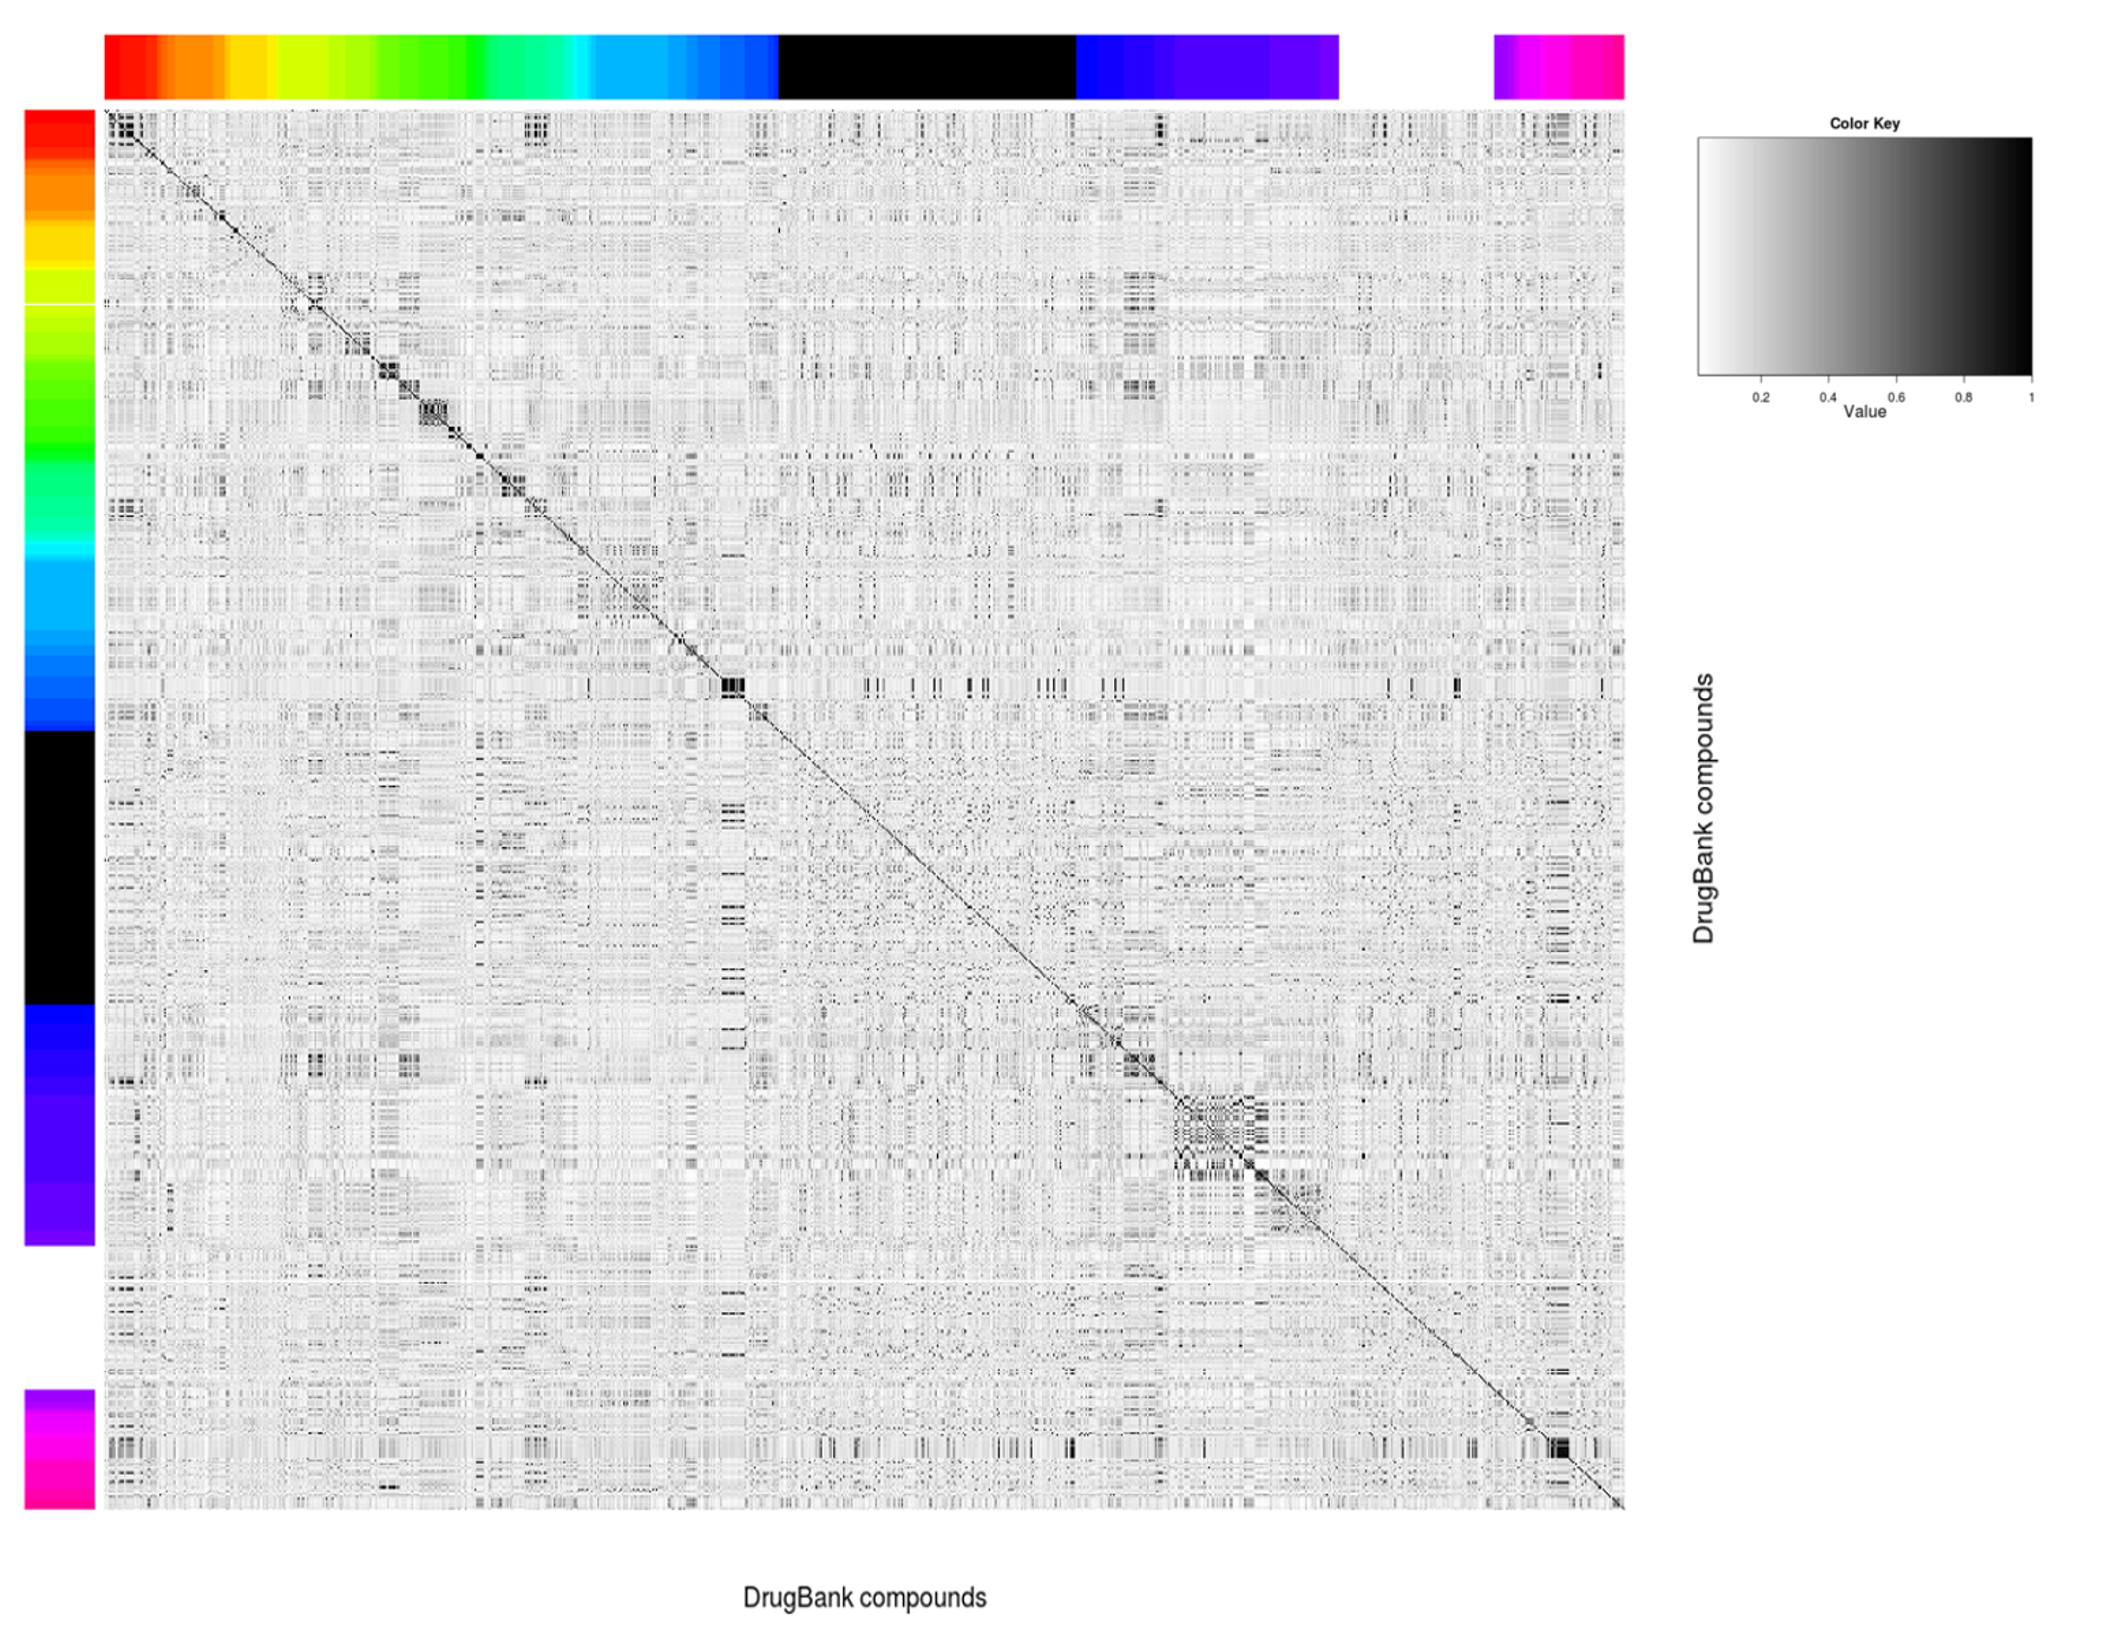
\includegraphics{figS3.png}}
\caption{Caption to be written.}\label{fig:S03}
\end{figure*}

\begin{figure*}[!tpb]%figureS4
\centerline{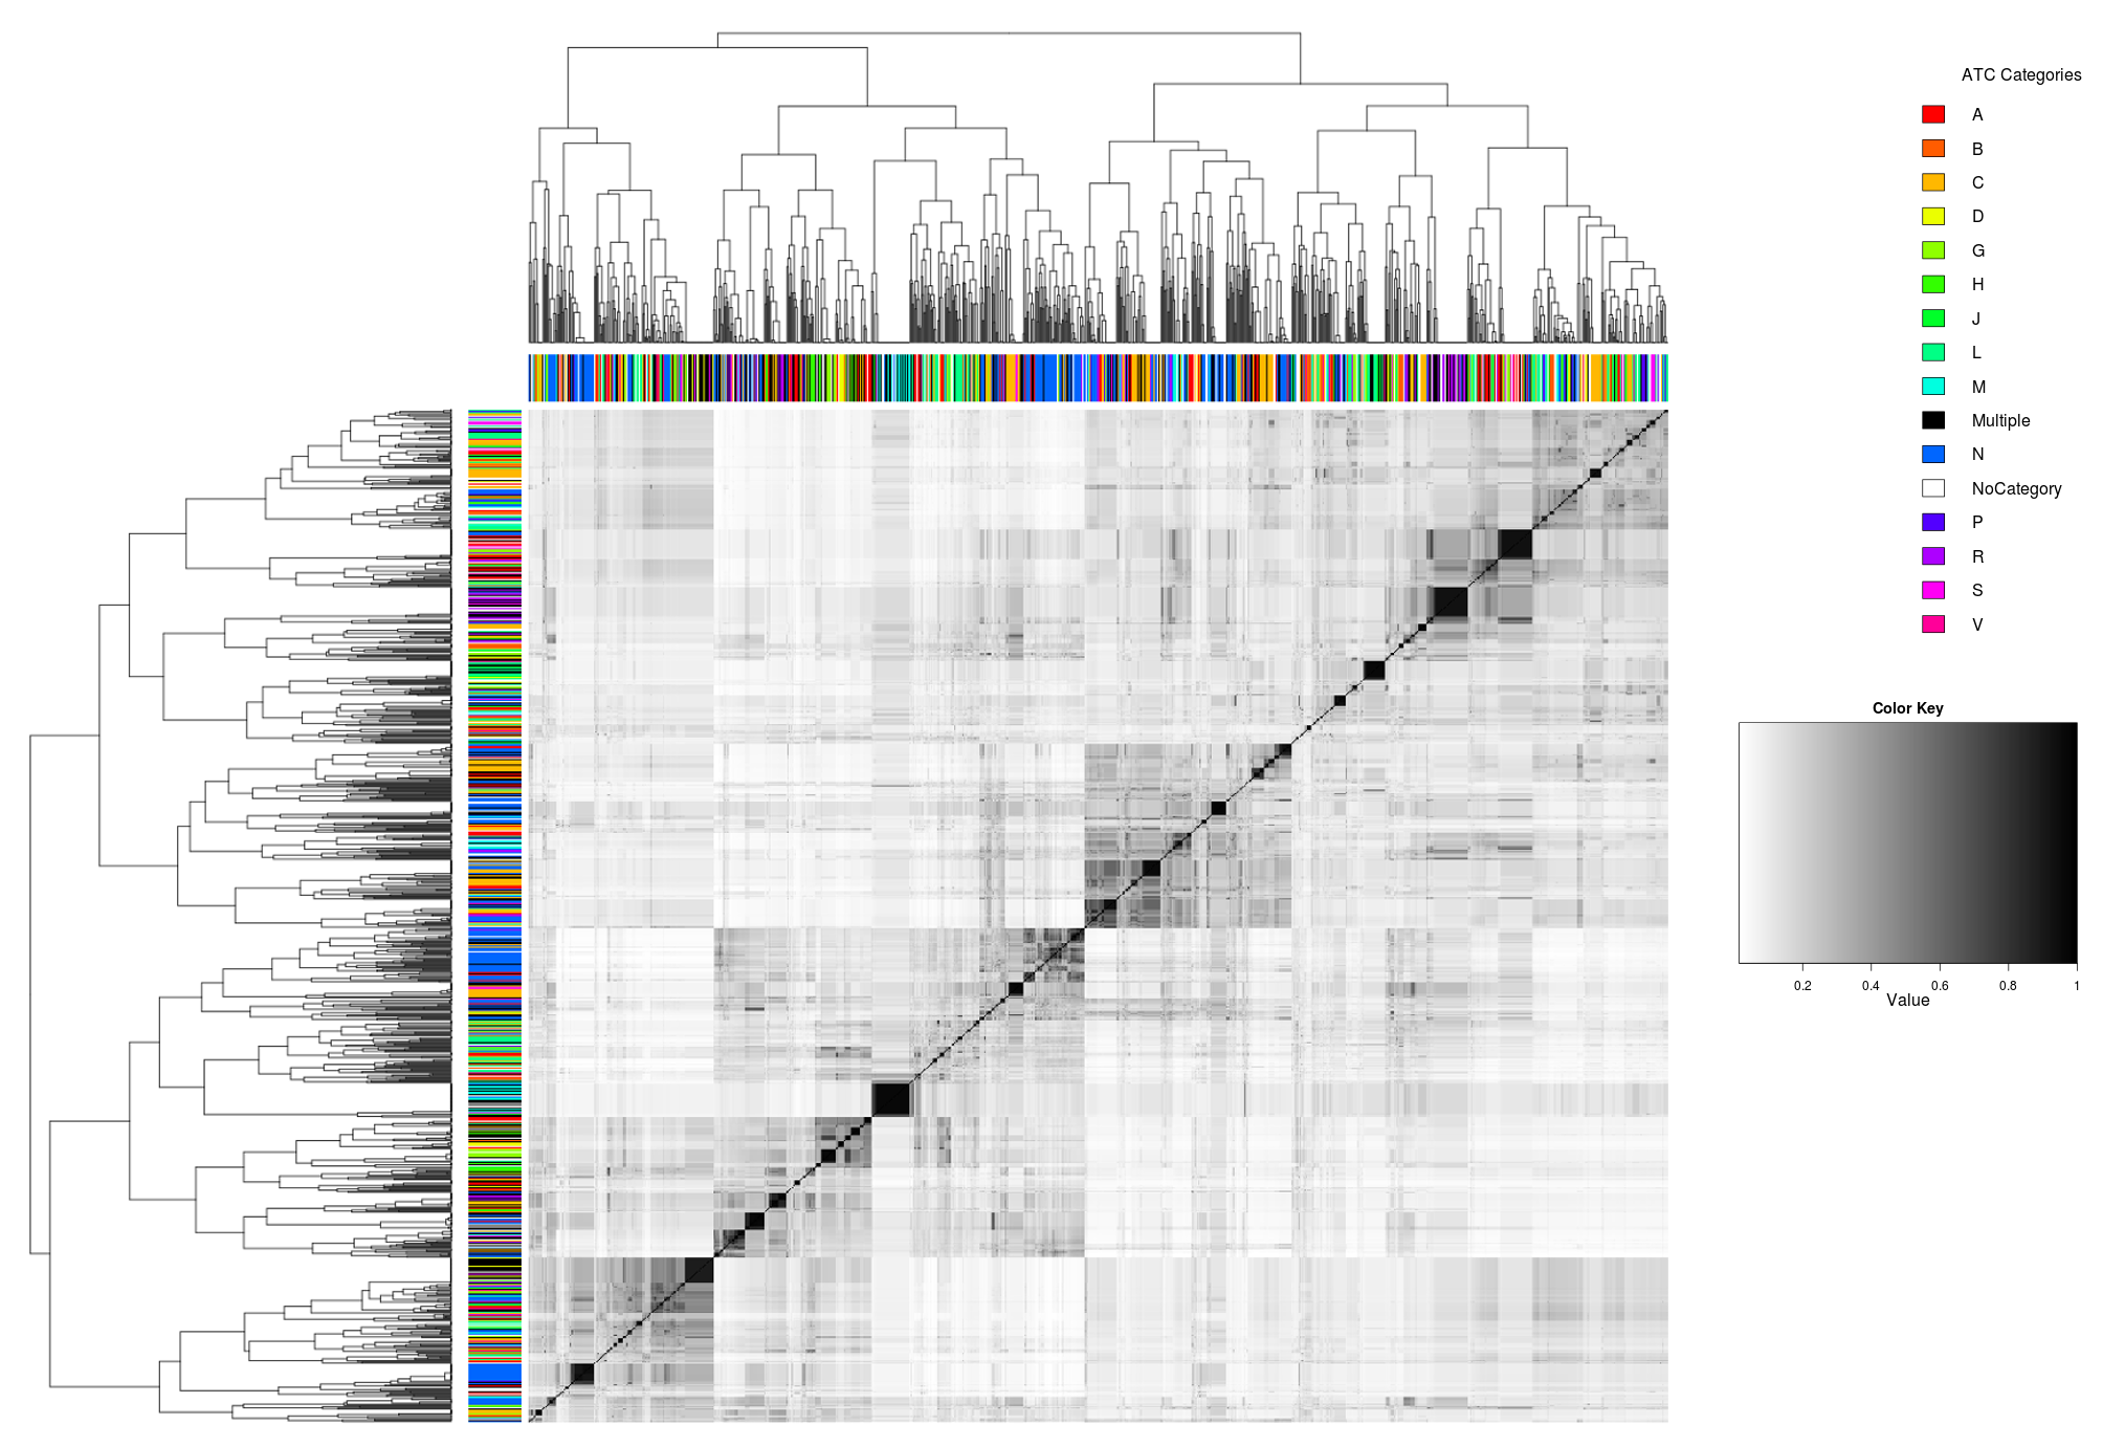
\includegraphics{figS4.png}}
\caption{Caption to be written.}\label{fig:S04}
\end{figure*}

\begin{figure*}[!tpb]%figureS5
\centerline{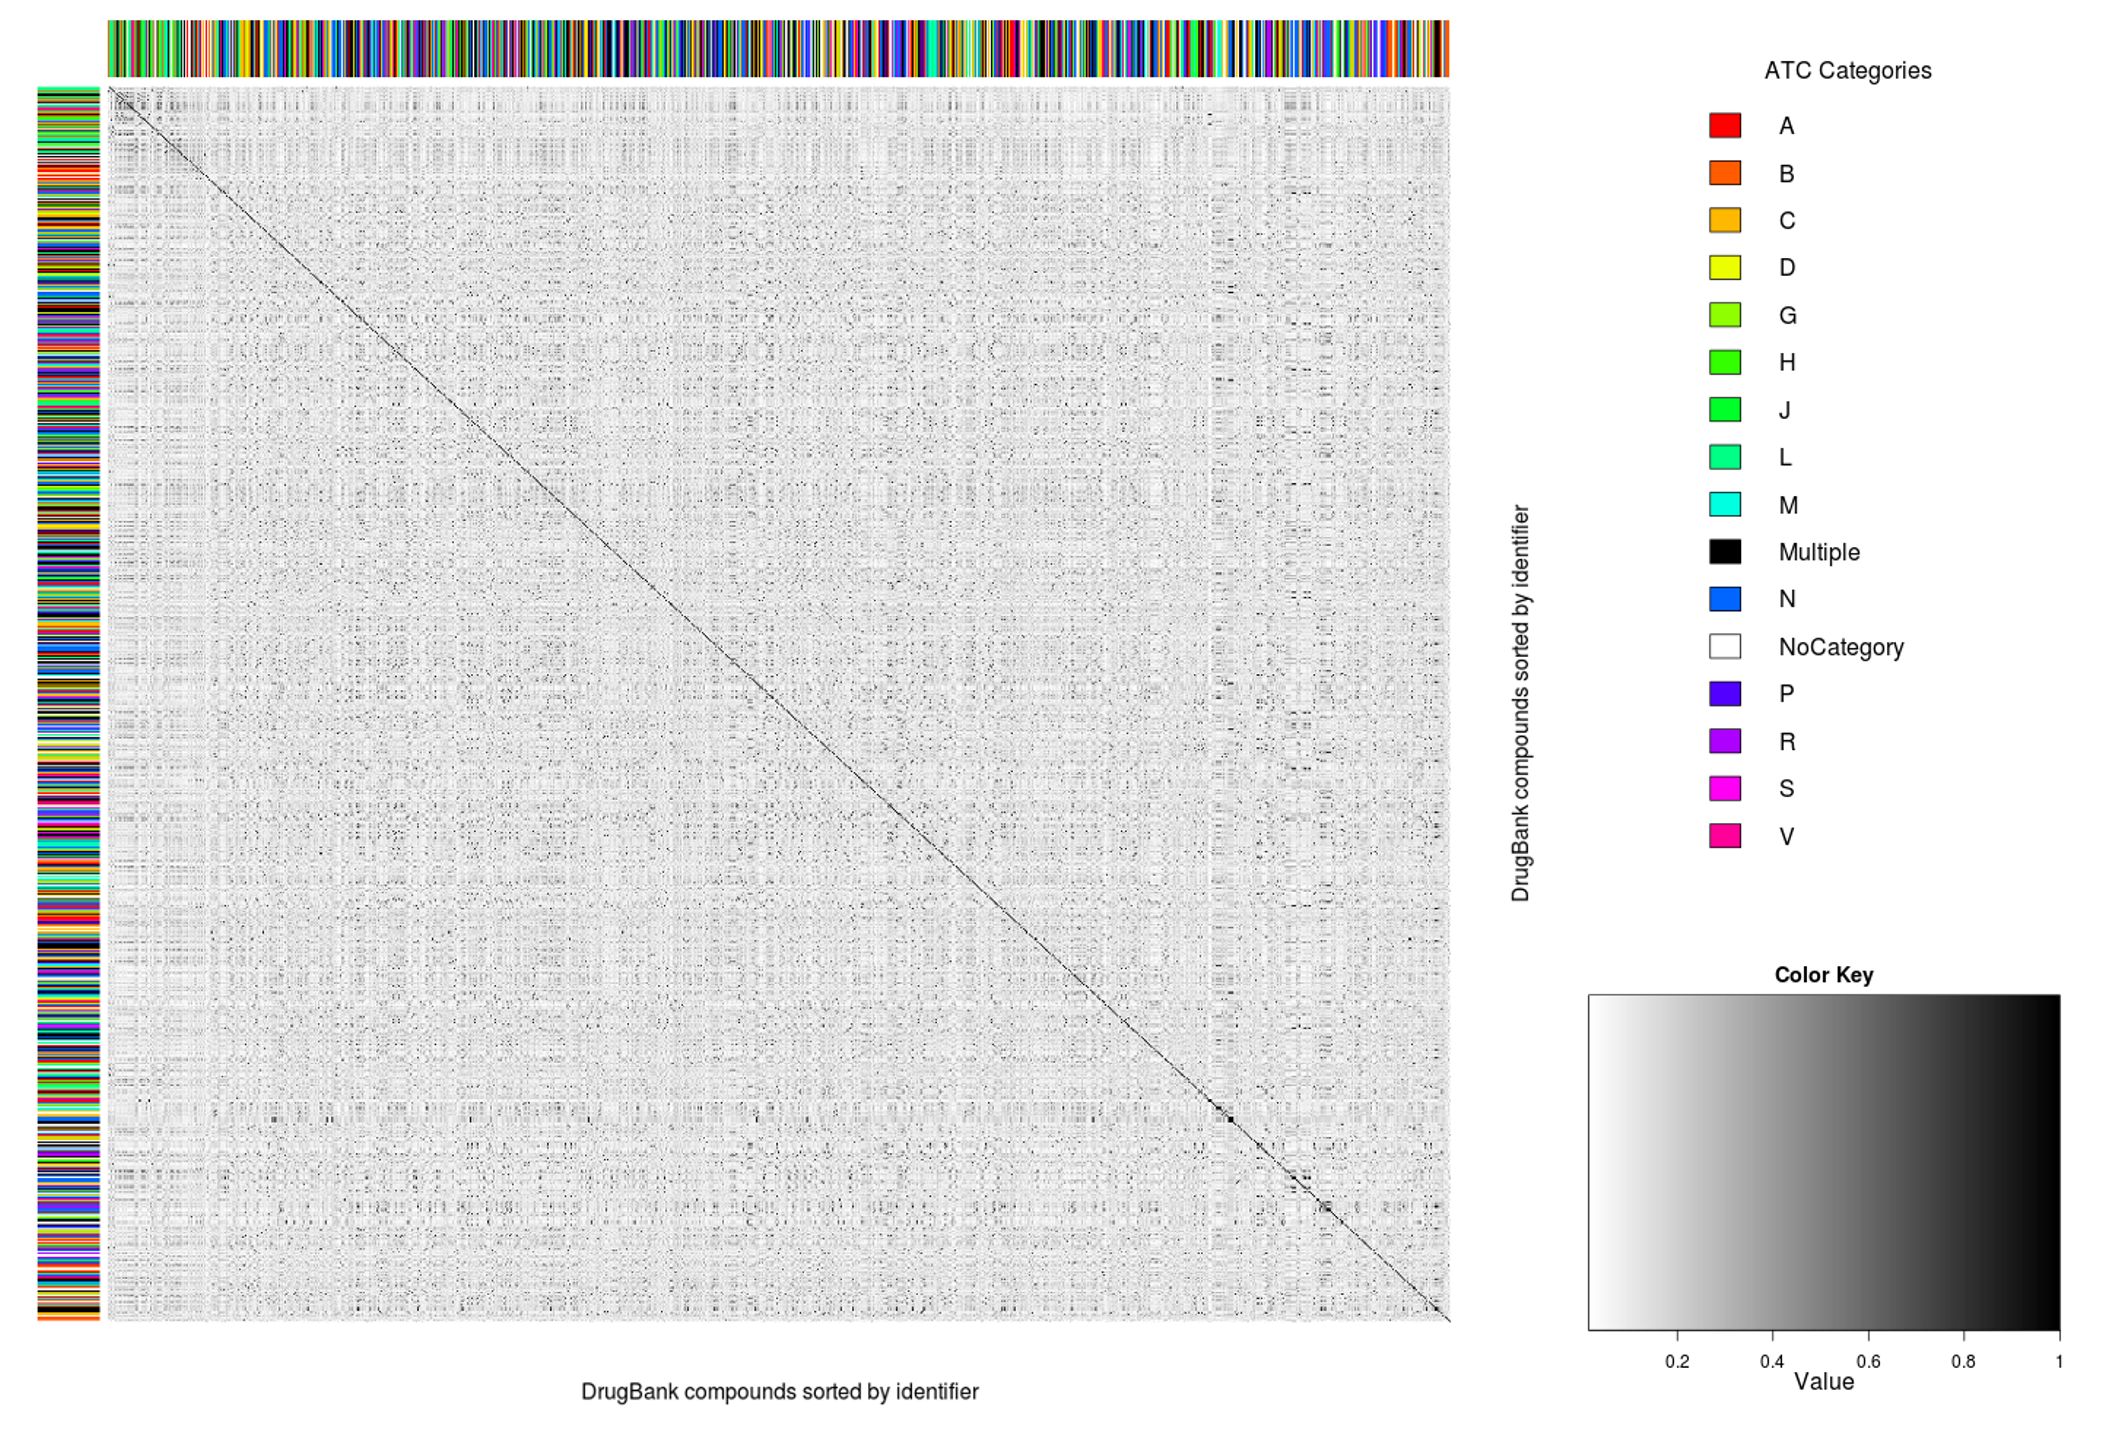
\includegraphics{figS5.png}}
\caption{Caption to be written.}\label{fig:S05}
\end{figure*}

\bibliographystyle{natbib}
\bibliographystyle{achemnat}
\bibliographystyle{plainnat}
\bibliographystyle{abbrv}
\bibliographystyle{bioinformatics}

\bibliographystyle{plain}

\bibliography{document}

\end{document}
